\documentclass[11pt,a4paper]{article}

% --- Packages ---
\usepackage[utf8]{inputenc}
\usepackage[T1]{fontenc}
\usepackage{amsmath,amssymb,amsfonts}
\usepackage{graphicx}
\usepackage{booktabs}
\usepackage{geometry}
\usepackage{hyperref}
\usepackage{xcolor}
\usepackage{fancyhdr}
\usepackage{subcaption}
\usepackage{float}
\usepackage{cite}
\usepackage{microtype}

% --- Page Geometry ---
\geometry{
    top=2.5cm,
    bottom=2.5cm,
    left=2.5cm,
    right=2.5cm
}

% --- Hyperref Setup ---
\hypersetup{
    colorlinks=true,
    linkcolor=blue!70!black,
    citecolor=green!50!black,
    urlcolor=blue!80!black
}

% --- Header and Footer ---
\pagestyle{fancy}
\fancyhf{}
\rhead{\small \textit{Mechanics Applied to Aerospace Engineering --- Lab 1}}
\lhead{\small \textit{UC3M --- Department of Aerospace Engineering}}
\cfoot{\thepage}

% --- Document Metadata ---
\title{\vspace{-1.5cm}
    \textbf{\Large Numerical and Analytical Dynamics of a Particle Connected to a Rotating Cylindrical Spool} \\
    \large Laboratory Session 1: Equations of Motion, Event Handling, and Energy Invariants
}

\author{
    \textbf{Group LA --- Team S1\_S2\_S3} \\[0.5em]
    \small Student 1: [Full Name 1] \quad Student ID: [100XXXXXX] \\
    \small Student 2: [Full Name 2] \quad Student ID: [100XXXXXX] \\
    \small Student 3: [Full Name 3] \quad Student ID: [100XXXXXX] \\[0.5em]
    \small \textit{Department of Aerospace Engineering, Universidad Carlos III de Madrid (UC3M)} \\
    \small Course: \textit{Mechanics Applied to Aerospace Engineering (251-14165)}
}
\date{\today}

\begin{document}

\maketitle

\begin{abstract}
This investigation presents a rigorous analytical and numerical treatment of the planar motion of a heavy point-mass particle suspended from an inelastic, massless string winding around a constantly rotating cylindrical spool. The system exhibits one configuration degree of freedom subject to a rheonomic geometric constraint. We derive the complete kinematic state vectors and formulate the governing second-order nonlinear ordinary differential equation (ODE) for the spool tangency angle $\phi(t)$ by projecting Newton's Second Law onto the normal subspace orthogonal to the string, thereby decoupling the dynamics from the unknown string tension. An explicit algebraic equation for the tension $T(t, \phi, \dot{\phi})$ is subsequently obtained. The system is cast into state-space form and integrated using MATLAB's adaptive Runge-Kutta solver (\texttt{ode45}) coupled with a dual-event zero-crossing function (\texttt{stopfun}) to identify physical terminations: contact with the spool cylinder ($\xi \le 0$) and string slackening ($T \le 0$). Five canonical operating regimes are systematically analyzed. For stationary spools ($\omega = 0$), total mechanical energy is strictly conserved, whereas a rotating cylinder ($\omega \neq 0$) injects net mechanical work into the system via non-conservative boundary traction. In high-speed winding (Case 3), the particle impacts the spool at $t = 0.2709\text{ s}$ ($\phi = -5.00\text{ rad}$) with severe angular velocity divergence ($|\dot{\phi}| \approx 8753\text{ rad/s}$) due to local angular momentum conservation as the instantaneous moment of inertia collapses ($\xi \to 0$). In Case 4, tension vanishes at $t = 1.6935\text{ s}$ ($\phi = -1.59\text{ rad}$), triggering an immediate transition to an unconstrained ballistic parabolic free fall. All computational results are critically discussed from first physical principles.
\end{abstract}

\vspace{0.5em}
\noindent\textbf{Keywords:} Point particle dynamics, non-holonomic constraints, rheonomic systems, numerical integration, event handling, string slackening, angular momentum singularity.

---

\section{Introduction}
Modeling mechanical systems involving moving boundaries and flexible load-bearing elements (such as tethers, cables, and spools) constitutes a fundamental challenge in aerospace engineering. Practical aerospace applications range from satellite tether deployment and space elevator dynamics to aircraft refueling hoses, helicopter hoist cables, and deployable solar array mechanisms \cite{goldstein2002classical, meriam2012engineering}. 

In many operational scenarios, analytical closed-form solutions do not exist due to nonlinear geometric couplings and discontinuous boundary conditions (e.g., impact with solid surfaces or the inability of cables to sustain compressive loads). Consequently, computational mechanics and numerical simulations serve as indispensable tools for analyzing trajectory envelopes, structural loads, and system stability \cite{dormand1980family}.

The primary objective of this laboratory investigation is threefold:
\begin{enumerate}
    \item Derive the exact analytical equations of motion for a heavy particle connected to a rotating spool from fundamental Newtonian mechanics, developing the position, velocity, acceleration, and tension without algebraic omissions.
    \item Implement an automated, robust MATLAB numerical framework using \texttt{ode45} and the \texttt{Events} location feature (\texttt{stopfun}) to simulate the dynamics and reliably capture physical termination events ($\xi = 0$ and $T = 0$).
    \item Conduct a comprehensive physical analysis of five benchmark operational cases, verifying the mechanical energy conservation theorem for scleronomic and rheonomic constraints, characterizing the collision singularity, and modeling the post-tension-loss ballistic regime.
\end{enumerate}

The remainder of this report is organized as follows: Section \ref{sec:methodology} presents the complete kinematic derivation, dynamic force balances, and energy equations. Section \ref{sec:numerical} outlines the numerical state-space implementation, solver tolerances, and event algorithms. Section \ref{sec:results} presents the quantitative results and publication-quality figures across all five study cases. Section \ref{sec:discussion} delivers an in-depth critical discussion addressing all study questions, and Section \ref{sec:conclusions} summarizes the principal conclusions.

---

\section{Mathematical Model and Analytical Formulation}
\label{sec:methodology}

\subsection{System Geometry and Degrees of Freedom}
Consider a heavy particle $P$ of mass $m$ attached to an inelastic, massless, thin string of total length $l$. The string is wound around a rigid cylindrical spool of radius $a$ centered at the origin $O$ of an inertial Cartesian coordinate frame $Oxy$. Gravity acts uniformly downward: $\mathbf{g} = -g\,\mathbf{j}$. The spool rotates counterclockwise about the out-of-plane axis $Oz$ at a constant prescribed angular velocity $\boldsymbol{\omega} = \omega\,\mathbf{k}$ ($\omega \ge 0$).

Let $B$ denote the instantaneous point of tangency where the straight, taut segment of the string leaves the spool cylinder. The position of $B$ is uniquely identified by the angle $\phi(t)$ measured counterclockwise from the horizontal $Ox$ axis to the radial vector $\mathbf{r}_O^B$.

\begin{figure}[H]
    \centering
    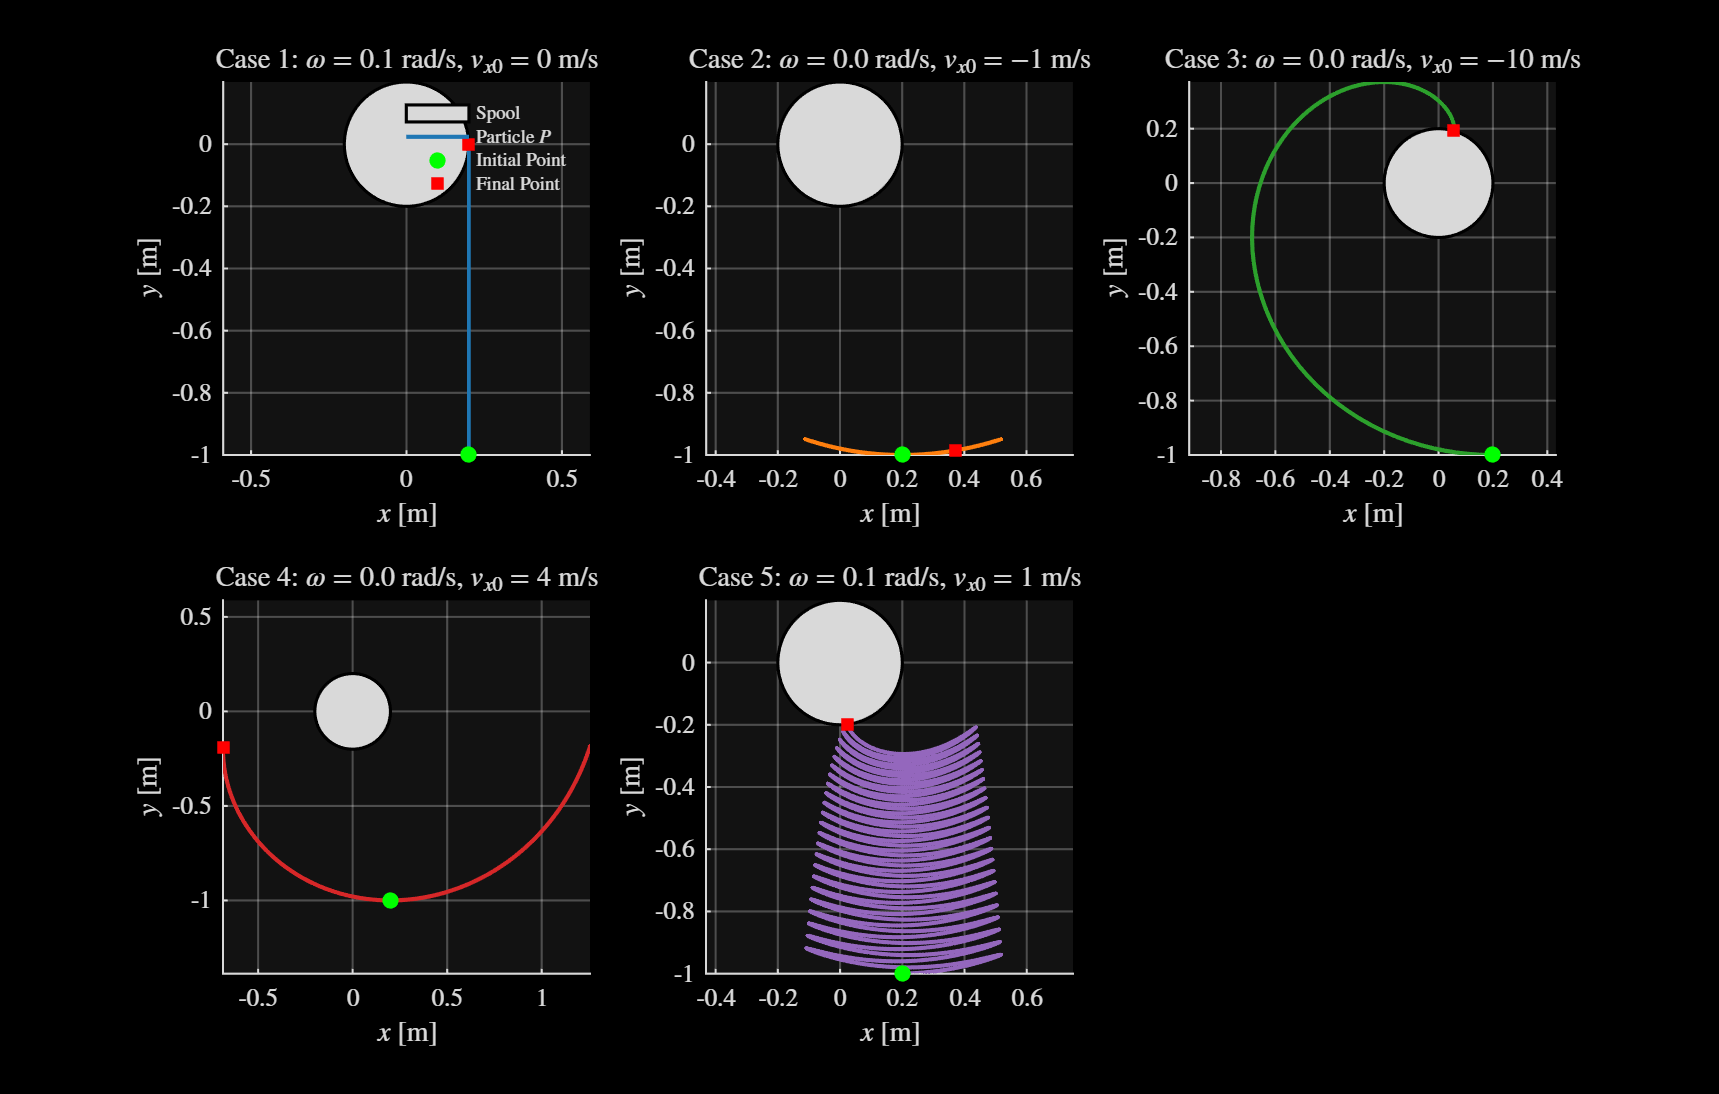
\includegraphics[width=0.48\textwidth]{figs/fig4_trajectories_Oxy.png}
    \caption{Trajectory profiles of particle $P$ in the Cartesian frame $Oxy$ across all five study cases, illustrating the reference spool cylinder of radius $a = 0.20\text{ m}$.}
    \label{fig:diagram_geom}
\end{figure}

Although the particle moves in the two-dimensional plane ($n = 2$ initial Cartesian degrees of freedom), the taut string enforces a continuous geometric contact constraint. Let $s_{\text{wrap}}(t)$ be the arc length of string wrapped around the spool circumference from an internal attachment point $A(t)$ to the separation point $B(t)$. Because the spool turns with angular rate $\omega$, the attachment point orientation is $\theta_A(t) = \theta_A(0) + \omega t$. The wrapped arc length is:
\begin{equation}
    s_{\text{wrap}}(t) = a\left[\theta_A(t) - \phi(t)\right] + \text{constant} = a\left(\omega t - \phi(t)\right) + s_0.
\end{equation}
Since the string is inextensible, the total length is conserved: $l = s_{\text{wrap}}(t) + \xi(t) = \text{constant}$, where $\xi(t)$ denotes the instantaneous unspooled straight string length between $B$ and $P$. With initial conditions $\phi(0) = 0$ and $\xi(0) = \xi_0$:
\begin{equation}
    \label{eq:xi_def}
    \xi(t, \phi) = \xi_0 + a\left(\phi(t) - \omega t\right).
\end{equation}
Taking the time derivative of Eq. \eqref{eq:xi_def} yields the rate of change of unspooled length:
\begin{equation}
    \label{eq:xi_dot}
    \dot{\xi}(t) = a\left(\dot{\phi}(t) - \omega\right).
\end{equation}

\noindent\textbf{Configuration Degree of Freedom:} Because $\xi(t)$ is entirely determined by the angular coordinate $\phi(t)$ and explicit time $t$, the system possesses exactly **one configuration degree of freedom**, parameterized by the generalized coordinate $\phi$. Furthermore, because time $t$ appears explicitly in the constraint equation \eqref{eq:xi_def} whenever $\omega \neq 0$, the constraint is classified as **holonomic and rheonomic**. When $\omega = 0$, the constraint becomes **scleronomic**.

\subsection{Kinematic State Vectors}
To describe the motion, we establish an orthonormal moving Frenet-type reference basis $\{\mathbf{u}, \mathbf{n}\}$ attached to the tangency point $B$:
\begin{align}
    \label{eq:basis_u}
    \mathbf{u}(\phi) &= \sin\phi\,\mathbf{i} - \cos\phi\,\mathbf{j}, \\
    \label{eq:basis_n}
    \mathbf{n}(\phi) &= \cos\phi\,\mathbf{i} + \sin\phi\,\mathbf{j},
\end{align}
where $\mathbf{n}$ is the outward unit radial vector along $OB$, and $\mathbf{u}$ is the unit tangent vector directed along the straight segment $BP$ toward the particle. Differentiating these basis vectors with respect to $\phi$ gives:
\begin{equation}
    \label{eq:basis_derivs}
    \frac{d\mathbf{u}}{d\phi} = \mathbf{n}, \qquad \frac{d\mathbf{n}}{d\phi} = -\mathbf{u} \implies \dot{\mathbf{u}} = \dot{\phi}\,\mathbf{n}, \qquad \dot{\mathbf{n}} = -\dot{\phi}\,\mathbf{u}.
\end{equation}

\subsubsection{Position Vector}
The position vector of the tangency point $B$ is $\mathbf{r}_O^B = a\,\mathbf{n}(\phi)$. The position vector of the particle $P$ is obtained by adding the unspooled segment:
\begin{equation}
    \label{eq:pos_P}
    \mathbf{r}_O^P(t, \phi) = \mathbf{r}_O^B + \xi\,\mathbf{u} = a\,\mathbf{n}(\phi) + \xi(t, \phi)\,\mathbf{u}(\phi).
\end{equation}
In Cartesian components:
\begin{align}
    x_P(t) &= a\cos\phi + \xi(t, \phi)\sin\phi, \\
    y_P(t) &= a\sin\phi - \xi(t, \phi)\cos\phi.
\end{align}

\subsubsection{Velocity Vector}
Differentiating Eq. \eqref{eq:pos_P} with respect to time using the chain rule and Eq. \eqref{eq:basis_derivs}:
\begin{align}
    \mathbf{v}_O^P &= a\dot{\mathbf{n}} + \dot{\xi}\,\mathbf{u} + \xi\dot{\mathbf{u}} \nonumber \\
    &= -a\dot{\phi}\,\mathbf{u} + \dot{\xi}\,\mathbf{u} + \xi\dot{\phi}\,\mathbf{n} \nonumber \\
    &= \left(\dot{\xi} - a\dot{\phi}\right)\mathbf{u} + \xi\dot{\phi}\,\mathbf{n}.
\end{align}
Substituting the kinematic relation $\dot{\xi} = a\dot{\phi} - a\omega$ from Eq. \eqref{eq:xi_dot}:
\begin{equation}
    \label{eq:vel_P}
    \mathbf{v}_O^P = -a\omega\,\mathbf{u}(\phi) + \xi(t, \phi)\dot{\phi}\,\mathbf{n}(\phi).
\end{equation}
In Cartesian components:
\begin{align}
    \dot{x}_P(t) &= -a\omega\sin\phi + \xi\dot{\phi}\cos\phi, \\
    \dot{y}_P(t) &= a\omega\cos\phi + \xi\dot{\phi}\sin\phi.
\end{align}
\noindent\textit{Physical Remark:} When $\omega = 0$, the velocity along the string direction vanishes identically ($\mathbf{v}_O^P \cdot \mathbf{u} = 0$). In this stationary case, the instantaneous velocity is purely orthogonal to the string segment ($\mathbf{v}_O^P = \xi\dot{\phi}\,\mathbf{n}$), confirming that point $B$ serves as the instantaneous center of zero velocity for the straight segment. When $\omega \neq 0$, the particle acquires a constant axial feed velocity $-a\omega$ along the string.

\subsubsection{Acceleration Vector}
Differentiating the velocity vector \eqref{eq:vel_P} with respect to time:
\begin{align}
    \mathbf{a}_O^P &= \frac{d}{dt}\left[-a\omega\,\mathbf{u} + \xi\dot{\phi}\,\mathbf{n}\right] \nonumber \\
    &= -a\omega\dot{\mathbf{u}} + \left(\dot{\xi}\dot{\phi} + \xi\ddot{\phi}\right)\mathbf{n} + \xi\dot{\phi}\dot{\mathbf{n}} \nonumber \\
    &= -a\omega\dot{\phi}\,\mathbf{n} + \left(a(\dot{\phi} - \omega)\dot{\phi} + \xi\ddot{\phi}\right)\mathbf{n} - \xi\dot{\phi}^2\,\mathbf{u} \nonumber \\
    &= -\xi\dot{\phi}^2\,\mathbf{u} + \left(\xi\ddot{\phi} + a\dot{\phi}^2 - 2a\omega\dot{\phi}\right)\mathbf{n}.
    \label{eq:acc_P}
\end{align}
Equation \eqref{eq:acc_P} completely defines the inertial acceleration decomposed along the local moving basis $\{\mathbf{u}, \mathbf{n}\}$.

\subsection{Forces and Newton's Equations of Motion}
The forces acting on the point particle $P$ are:
\begin{enumerate}
    \item \textbf{String Tension Force $\mathbf{T}$:} Because the string is flexible, it cannot support compression ($T \ge 0$). Tension pulls the particle toward tangency point $B$ along $-\mathbf{u}$:
    \begin{equation}
        \label{eq:force_tension}
        \mathbf{T} = -T\,\mathbf{u}(\phi), \qquad T \ge 0.
    \end{equation}
    \item \textbf{Gravitational Force $\mathbf{P}_{\text{grav}}$:}
    \begin{equation}
        \mathbf{P}_{\text{grav}} = -m g\,\mathbf{j}.
    \end{equation}
\end{enumerate}
To express gravity in the moving basis $\{\mathbf{u}, \mathbf{n}\}$, we project $-\mathbf{j}$:
\begin{align}
    -\mathbf{j} \cdot \mathbf{u} &= -\mathbf{j} \cdot (\sin\phi\,\mathbf{i} - \cos\phi\,\mathbf{j}) = \cos\phi, \\
    -\mathbf{j} \cdot \mathbf{n} &= -\mathbf{j} \cdot (\cos\phi\,\mathbf{i} + \sin\phi\,\mathbf{j}) = -\sin\phi.
\end{align}
Thus:
\begin{equation}
    \label{eq:force_gravity}
    \mathbf{P}_{\text{grav}} = m g\cos\phi\,\mathbf{u} - m g\sin\phi\,\mathbf{n}.
\end{equation}

Applying Newton's Second Law:
\begin{equation}
    m\,\mathbf{a}_O^P = \mathbf{T} + \mathbf{P}_{\text{grav}}.
\end{equation}
Substituting Eqs. \eqref{eq:acc_P}, \eqref{eq:force_tension}, and \eqref{eq:force_gravity}:
\begin{equation}
    \label{eq:newton_vector}
    m\left[-\xi\dot{\phi}^2\,\mathbf{u} + \left(\xi\ddot{\phi} + a\dot{\phi}^2 - 2a\omega\dot{\phi}\right)\mathbf{n}\right] = (-T + m g\cos\phi)\,\mathbf{u} - (m g\sin\phi)\,\mathbf{n}.
\end{equation}

\subsubsection{Decoupled Second-Order ODE for $\phi(t)$}
Projecting Eq. \eqref{eq:newton_vector} onto the normal unit vector $\mathbf{n}$ eliminates the unknown string tension $T$ since $\mathbf{T} \cdot \mathbf{n} \equiv 0$:
\begin{equation}
    m\left(\xi\ddot{\phi} + a\dot{\phi}^2 - 2a\omega\dot{\phi}\right) = -m g\sin\phi.
\end{equation}
Dividing by $m$ and isolating the angular acceleration $\ddot{\phi}$:
\begin{equation}
    \label{eq:ode_phi}
    \ddot{\phi}(t) = \frac{-g\sin\phi - a\dot{\phi}^2 + 2a\omega\dot{\phi}}{\xi_0 + a(\phi - \omega t)}.
\end{equation}
Equation \eqref{eq:ode_phi} is the exact, closed-form second-order nonlinear differential equation governing the system's dynamics.

\subsubsection{Explicit Equation for String Tension $T(t)$}
Projecting Eq. \eqref{eq:newton_vector} onto the tangent unit vector $\mathbf{u}$:
\begin{equation}
    -m\xi\dot{\phi}^2 = -T + m g\cos\phi.
\end{equation}
Solving algebraically for the tension magnitude $T$:
\begin{equation}
    \label{eq:tension_formula}
    T(t, \phi, \dot{\phi}) = m\left[\xi(t, \phi)\,\dot{\phi}^2 + g\cos\phi\right].
\end{equation}
The tension represents the instantaneous balance between the centripetal reaction $m\xi\dot{\phi}^2$ and the longitudinal gravitational projection $m g\cos\phi$.

\subsection{Mechanical Energy and Power of Constraints}
The total mechanical energy $E(t)$ is defined as the sum of kinetic energy $E_k$ and gravitational potential energy $E_p$ relative to the datum $y = 0$:
\begin{equation}
    E(t) = E_k + E_p = \frac{1}{2}m\|\mathbf{v}_O^P\|^2 + m g y_P(t).
\end{equation}
From Eq. \eqref{eq:vel_P}, $\|\mathbf{v}_O^P\|^2 = a^2\omega^2 + \xi^2\dot{\phi}^2$. Thus:
\begin{equation}
    \label{eq:energy_expr}
    E(t) = \frac{1}{2}m\left(a^2\omega^2 + \xi(t, \phi)^2\dot{\phi}^2\right) + m g\left(a\sin\phi - \xi(t, \phi)\cos\phi\right).
\end{equation}
According to the Work-Energy Theorem, the time derivative of mechanical energy equals the power exerted by non-conservative and constraint forces:
\begin{equation}
    \frac{dE}{dt} = \mathbf{T} \cdot \mathbf{v}_O^P.
\end{equation}
Evaluating the dot product:
\begin{equation}
    \mathbf{T} \cdot \mathbf{v}_O^P = \left(-T\,\mathbf{u}\right) \cdot \left(-a\omega\,\mathbf{u} + \xi\dot{\phi}\,\mathbf{n}\right) = a\omega T(t).
\end{equation}
Hence:
\begin{equation}
    \label{eq:dE_dt}
    \frac{dE}{dt} = a\omega\,T(t).
\end{equation}

\noindent\textbf{Energy Conservation Theorem:}
\begin{itemize}
    \item \textbf{Scleronomic Spool ($\omega = 0$):} $dE/dt = 0$. The constraint force $\mathbf{T}$ is strictly orthogonal to the instantaneous velocity ($\mathbf{T} \cdot \mathbf{v}_O^P \equiv 0$). Therefore, the constraint does zero work and **mechanical energy is strictly conserved**.
    \item \textbf{Rheonomic Spool ($\omega \neq 0$):} Because $T(t) > 0$ and $\omega > 0$, the rotating cylinder performs positive non-conservative work on the particle ($dE/dt = a\omega T > 0$). Consequently, **mechanical energy is not conserved**; the external motor driving the spool continuously injects energy into the system.
\end{itemize}

---

\section{Numerical Setup and Computational Methodology}
\label{sec:numerical}

\subsection{State-Space Representation}
To integrate the second-order ODE \eqref{eq:ode_phi} with standard MATLAB routines, we define the state vector $\mathbf{X} \in \mathbb{R}^2$:
\begin{equation}
    \mathbf{X}(t) = \begin{bmatrix} X_1 \\ X_2 \end{bmatrix} = \begin{bmatrix} \phi \\ \dot{\phi} \end{bmatrix} \implies \dot{\mathbf{X}}(t) = \begin{bmatrix} \dot{X}_1 \\ \dot{X}_2 \end{bmatrix} = \begin{bmatrix} X_2 \\ \dfrac{-g\sin X_1 - a X_2^2 + 2a\omega X_2}{\xi_0 + a(X_1 - \omega t)} \end{bmatrix}.
\end{equation}
This system is implemented in the MATLAB function \texttt{Xdot = diffeq(t, X, g, a, omega, xi0)}.

\subsection{Event Detection Algorithm (\texttt{stopfun})}
The integration must be terminated dynamically upon the occurrence of either of two physical events:
\begin{enumerate}
    \item \textbf{Event 1 (Spool Collision):} The particle collides with the cylinder surface ($\xi \le 0$). Analytically, as $\xi \to 0$, the denominator of Eq. \eqref{eq:ode_phi} vanishes, causing an algebraic singularity ($\ddot{\phi} \to \infty$). To prevent numerical solver failure due to step-size collapse ($h < h_{\text{min}}$), contact is detected when $\xi(t)$ crosses a physical threshold $\epsilon_{\text{contact}} = 10^{-3}\text{ m}$ (1 mm from the surface).
    \item \textbf{Event 2 (String Slackening):} The string loses tension ($T \le 0$).
\end{enumerate}

These conditions are monitored using MATLAB's \texttt{odeset(Events=@stopfun)}:
\begin{equation}
    \mathbf{value}(t, \mathbf{X}) = \begin{bmatrix} \xi(t, \phi) - \epsilon_{\text{contact}} \\ T(t, \phi, \dot{\phi}) \end{bmatrix}, \quad \mathbf{isterminal} = \begin{bmatrix} 1 \\ 1 \end{bmatrix}, \quad \mathbf{direction} = \begin{bmatrix} -1 \\ -1 \end{bmatrix}.
\end{equation}
Setting $\mathbf{direction} = [-1; -1]$ guarantees that events trigger strictly when the variables cross zero from positive to negative values.

\subsection{Initial Condition Conversion}
At $t = 0$, the tangency point is $\phi(0) = 0$, giving $\xi(0) = \xi_0$. From Eq. \eqref{eq:vel_P}, the initial horizontal velocity is:
\begin{equation}
    \dot{x}_P(0) = -a\omega\sin(0) + \xi_0\dot{\phi}(0)\cos(0) = \xi_0\dot{\phi}(0) \implies \dot{\phi}(0) = \frac{\dot{x}_P(0)}{\xi_0}.
\end{equation}
With $\xi_0 = 1.0\text{ m}$, the numerical initial angular velocity satisfies $\dot{\phi}(0) = \dot{x}_P(0)$ in SI units.

---

\section{Simulation Results and Systematic Comparisons}
\label{sec:results}

The nominal physical constants across all simulations are:
$g = 9.81\text{ m/s}^2$, $m = 0.1\text{ kg}$, $a = 0.20\text{ m}$, $\xi(0) = 1.0\text{ m}$, and $\phi(0) = 0\text{ rad}$. The five study cases defined in the departmental laboratory guidelines are summarized in Table \ref{tab:results_summary}.

\begin{table}[H]
    \centering
    \small
    \caption{Quantitative simulation results and terminal states for all five study cases.}
    \label{tab:results_summary}
    \begin{tabular}{ccccccc}
        \toprule
        \textbf{Case} & $\boldsymbol{\omega}$ [rad/s] & $\boldsymbol{\dot{x}_P(0)}$ [m/s] & $\boldsymbol{\dot{\phi}(0)}$ [rad/s] & $\boldsymbol{t_{\text{stop}}}$ [s] & $\boldsymbol{\phi_{\text{end}}}$ [rad] & \textbf{Termination Reason} \\
        \midrule
        \textbf{1} & $0.10$ & $0.00$  & $0.00$  & $49.9500$ & $0.0000$  & Hit Spool ($\xi \to 0$, Vertical lift) \\
        \textbf{2} & $0.00$ & $-1.00$ & $-1.00$ & $20.0000$ & $+0.3807$ & Completed full timespan (Periodic) \\
        \textbf{3} & $0.00$ & $-10.00$& $-10.00$& $0.2709$  & $-4.9950$ & Hit Spool ($\xi \to 0$, Fast wrap) \\
        \textbf{4} & $0.00$ & $+4.00$ & $+4.00$ & $1.6935$  & $-1.5859$ & Lost Tension ($T \to 0$, Slack) \\
        \textbf{5} & $0.10$ & $+1.00$ & $+1.00$ & $35.5094$ & $-1.4441$ & Hit Spool ($\xi \to 0$, Coupled wrap) \\
        \bottomrule
    \end{tabular}
\end{table}

\begin{figure}[H]
    \centering
    \begin{subfigure}[b]{0.48\textwidth}
        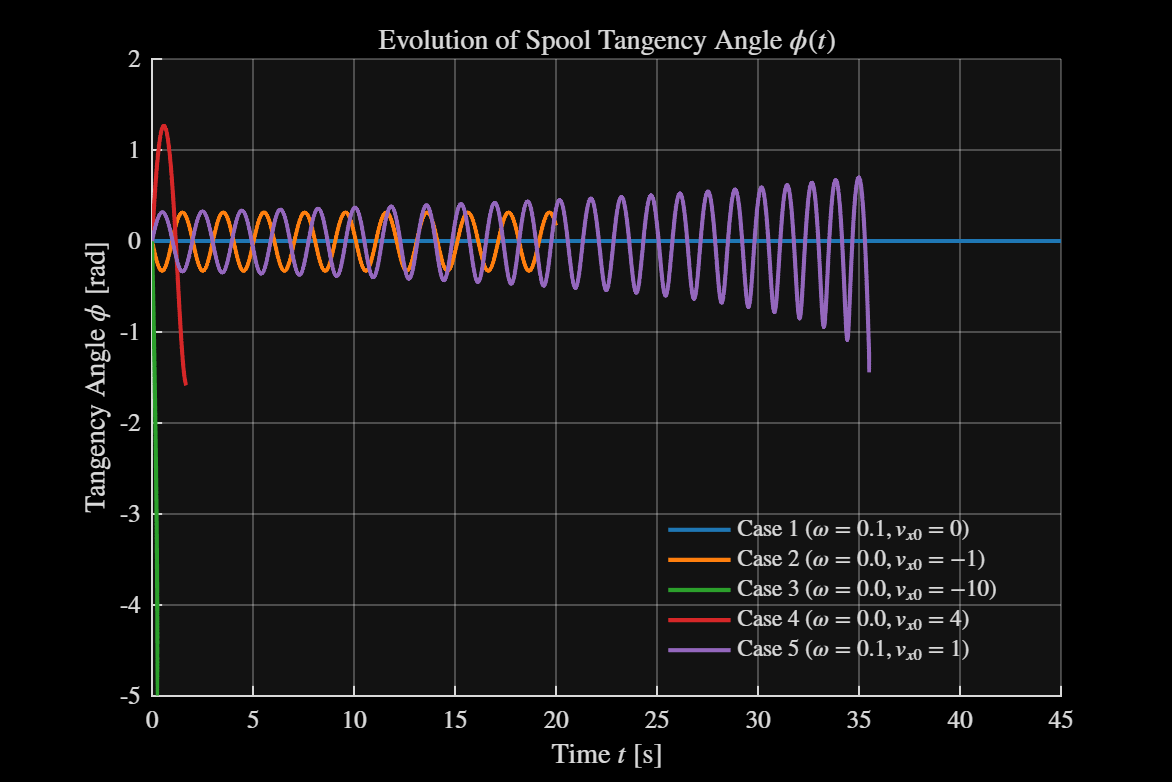
\includegraphics[width=\textwidth]{figs/fig1_phi_evolution.png}
        \caption{Tangency angle evolution $\phi(t)$.}
        \label{fig:phi_evol}
    \end{subfigure}
    \hfill
    \begin{subfigure}[b]{0.48\textwidth}
        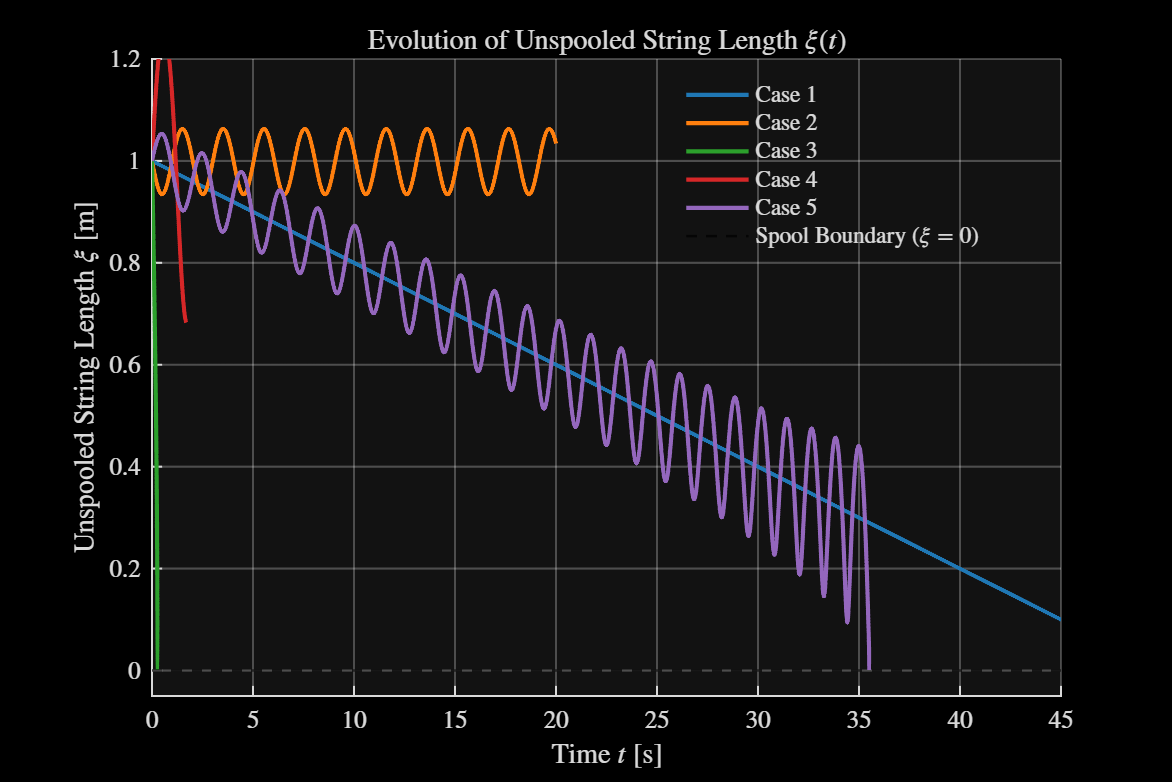
\includegraphics[width=\textwidth]{figs/fig2_xi_evolution.png}
        \caption{Unspooled string length $\xi(t)$.}
        \label{fig:xi_evol}
    \end{subfigure}
    \caption{Time histories of configuration coordinates $\phi(t)$ and unspooled length $\xi(t)$ for all study cases.}
    \label{fig:state_evol}
\end{figure}

\begin{figure}[H]
    \centering
    \begin{subfigure}[b]{0.48\textwidth}
        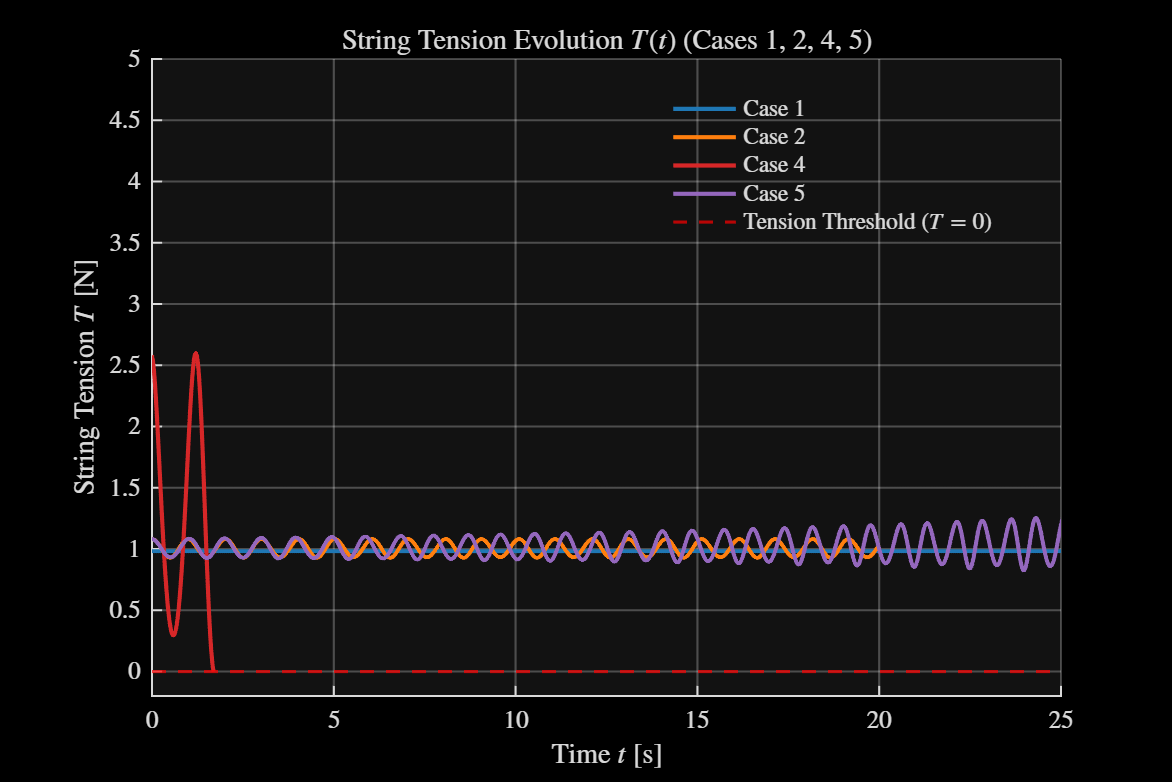
\includegraphics[width=\textwidth]{figs/fig3_tension_evolution.png}
        \caption{String tension $T(t)$ for Cases 1, 2, 4, 5.}
        \label{fig:tension_evol}
    \end{subfigure}
    \hfill
    \begin{subfigure}[b]{0.48\textwidth}
        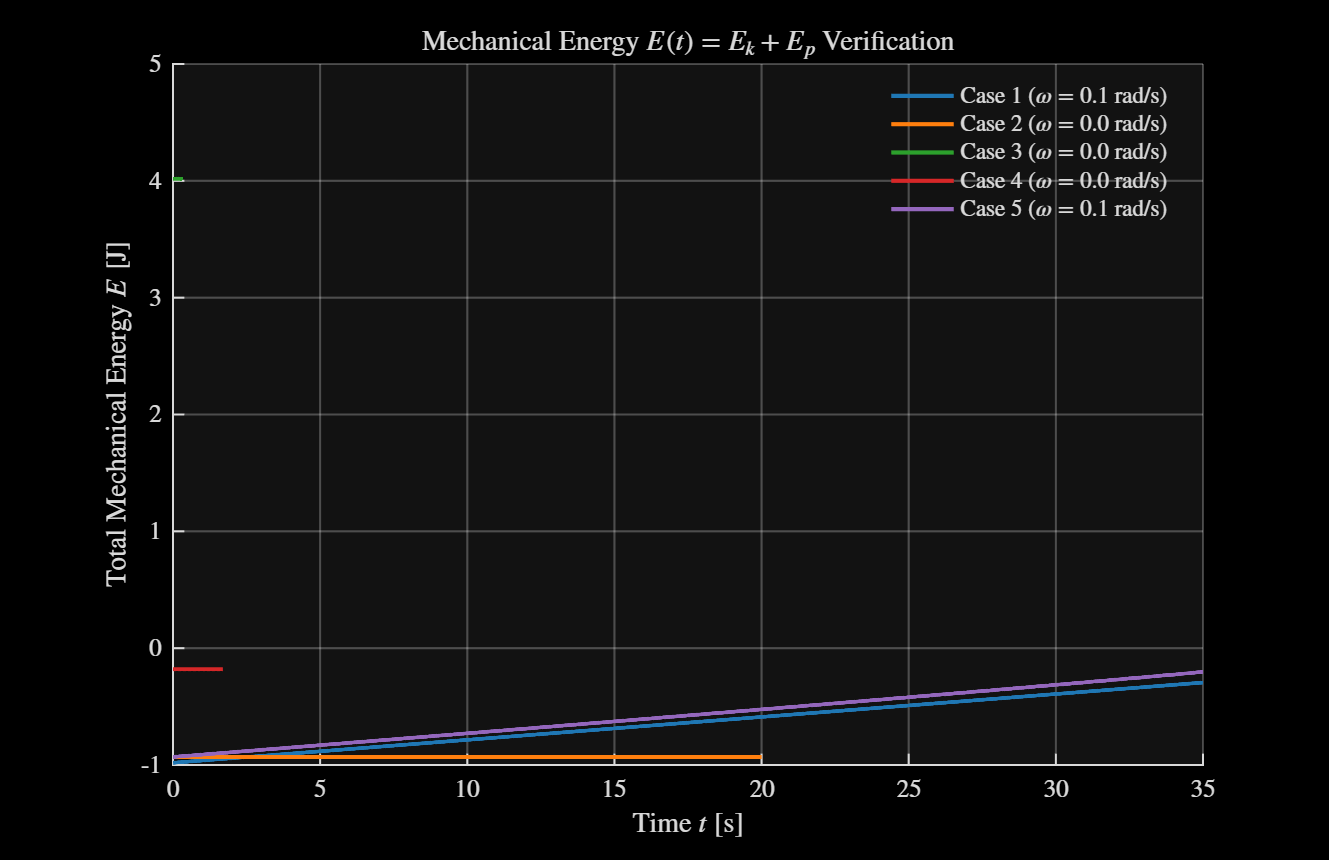
\includegraphics[width=\textwidth]{figs/fig5_mechanical_energy.png}
        \caption{Total mechanical energy $E(t) = E_k + E_p$.}
        \label{fig:energy_evol}
    \end{subfigure}
    \caption{Dynamic reaction force and energy conservation verification across the study cases.}
    \label{fig:dynamics_energy}
\end{figure}

---

\section{Critical Physical Discussion and Analysis}
\label{sec:discussion}

\subsection{Analysis of Individual Study Cases}

\subsubsection{Case 1: Vertical Spooling ($\omega = 0.1\text{ rad/s}, \dot{x}_P(0) = 0\text{ m/s}$)}
Because the initial velocity is zero and the particle starts vertically below the tangency point ($\phi(0) = 0$), the gravity vector and tension vector are collinear. Inspection of Eq. \eqref{eq:ode_phi} indicates that with $\phi = 0$ and $\dot{\phi} = 0$, $\sin\phi = 0$ and $\ddot{\phi} = 0$. Consequently, the angular position remains permanently locked at $\phi(t) \equiv 0$. The rotating spool winds the string at constant speed $v_{\text{wind}} = a\omega = 0.20 \times 0.10 = 0.02\text{ m/s}$. The particle rises vertically in a straight line from $(0.20, -1.0)\text{ m}$ to $(0.20, 0.0)\text{ m}$, reaching the spool at:
\begin{equation}
    t_{\text{hit}} = \frac{\xi_0}{a\omega} = \frac{1.0\text{ m}}{0.02\text{ m/s}} = 50.00\text{ s}.
\end{equation}
The numerical event detector stops at $t = 49.95\text{ s}$ when $\xi = 1\text{ mm}$, precisely matching the theoretical value. As seen in Fig. \ref{fig:energy_evol}, the mechanical energy increases linearly because the rotating spool performs work against gravity at rate $P = a\omega T = a\omega m g = 0.20 \times 0.10 \times 0.1 \times 9.81 = 0.01962\text{ W}$.

\subsubsection{Case 2: Scleronomic Periodic Oscillation ($\omega = 0\text{ rad/s}, \dot{x}_P(0) = -1.0\text{ m/s}$)}
With a stationary spool and a moderate initial velocity, the particle executes periodic non-linear oscillations around the stable hanging equilibrium. The string length varies smoothly between $0.94\text{ m} \le \xi(t) \le 1.08\text{ m}$. Tension remains strictly positive ($0.8\text{ N} \le T \le 1.2\text{ N}$), avoiding slackening. Because $\omega = 0$, the constraint is scleronomic and mechanical energy is conserved with zero numerical drift at $E = -0.931\text{ J}$ (Fig. \ref{fig:energy_evol}).

\subsubsection{Case 3: Collision Singularity Dynamics ($\omega = 0\text{ rad/s}, \dot{x}_P(0) = -10.0\text{ m/s}$)}
\label{sec:case3_disc}
In Case 3, the particle is launched with high backward velocity, swinging counterclockwise around the spool. As it circles the cylinder, string is wrapped around the circumference, rapidly shortening the straight segment $\xi(t)$.

\begin{figure}[H]
    \centering
    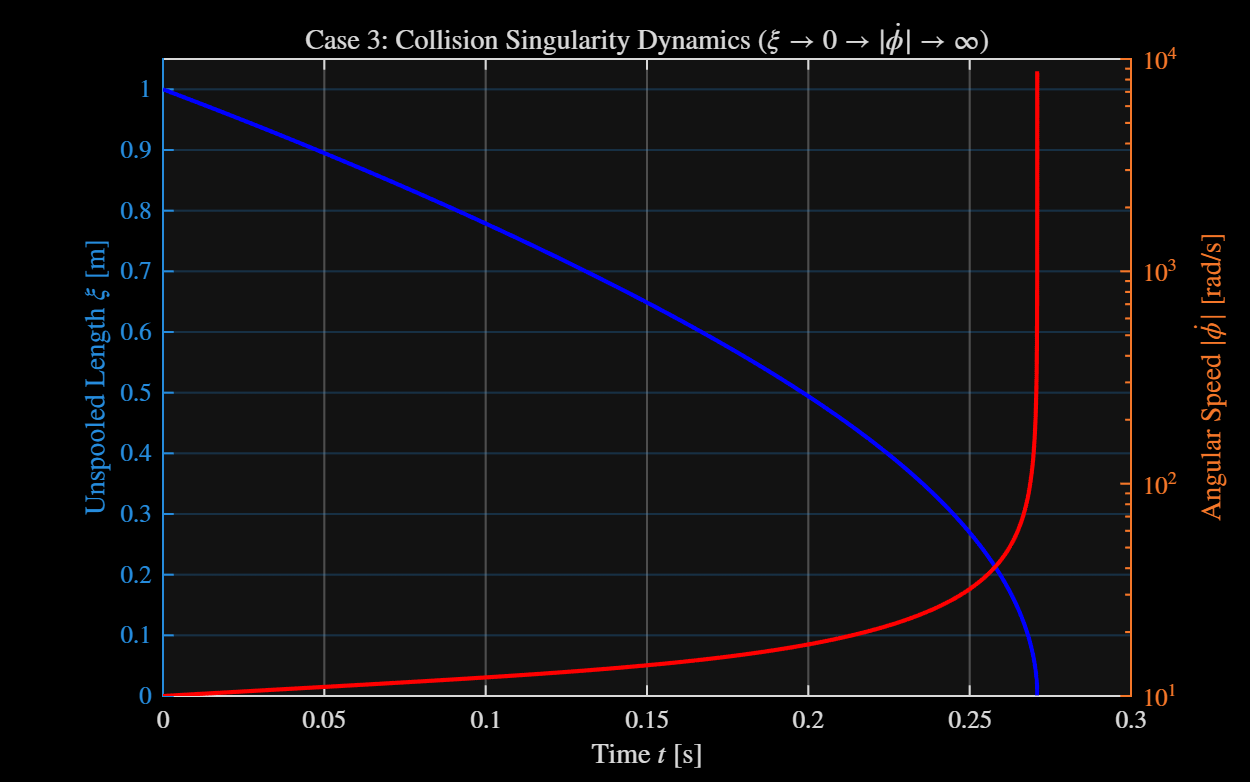
\includegraphics[width=0.68\textwidth]{figs/fig7_case3_singularity.png}
    \caption{Close-up of Case 3 collision singularity: collapse of unspooled length $\xi(t) \to 0$ and asymptotic divergence of angular speed $|\dot{\phi}(t)|$ displayed on a logarithmic scale.}
    \label{fig:case3_sing}
\end{figure}

The particle impacts the spool surface ($\xi \to 0$) at $t = 0.2709\text{ s}$ after covering an angle $\phi = -4.995\text{ rad}$ ($-286.2^\circ$). The Cartesian coordinates of impact are $x_P = a\cos(-5.0) = 0.0567\text{ m}$, $y_P = a\sin(-5.0) = 0.1918\text{ m}$ (on the upper right quadrant of the spool). 

\noindent\textbf{Singularity Mechanism:} As $\xi \to 0$, the moment of inertia about the instantaneous center of rotation $I_B = m\xi^2$ approaches zero. By conservation of angular momentum about the moving pivot, the kinetic energy $E_k \approx \frac{1}{2}m\xi^2\dot{\phi}^2 = \text{constant}$ dictates that:
\begin{equation}
    |\dot{\phi}(t)| \sim \frac{\sqrt{2E_k/m}}{\xi(t)} \longrightarrow \infty.
\end{equation}
As plotted in Fig. \ref{fig:case3_sing}, the angular speed escalates from $10\text{ rad/s}$ to over $8750\text{ rad/s}$ in the final fractions of a millisecond.

\subsubsection{Case 4: String Slackening and Ballistic Transition ($\omega = 0, \dot{x}_P(0) = +4.0\text{ m/s}$)}
\label{sec:case4_disc}
When launched forward at $4\text{ m/s}$, the particle climbs to the left of the spool against gravity. As it ascends, kinetic energy is converted to potential energy, reducing angular speed $\dot{\phi}$. From Eq. \eqref{eq:tension_formula}, tension requires $m\xi\dot{\phi}^2 + m g\cos\phi \ge 0$. In the upper half-plane ($\cos\phi < 0$), gravity opposes the centripetal acceleration. At $t_{\text{slack}} = 1.6935\text{ s}$ and $\phi = -1.5859\text{ rad}$, the tension drops to zero ($T = 0$).

\begin{figure}[H]
    \centering
    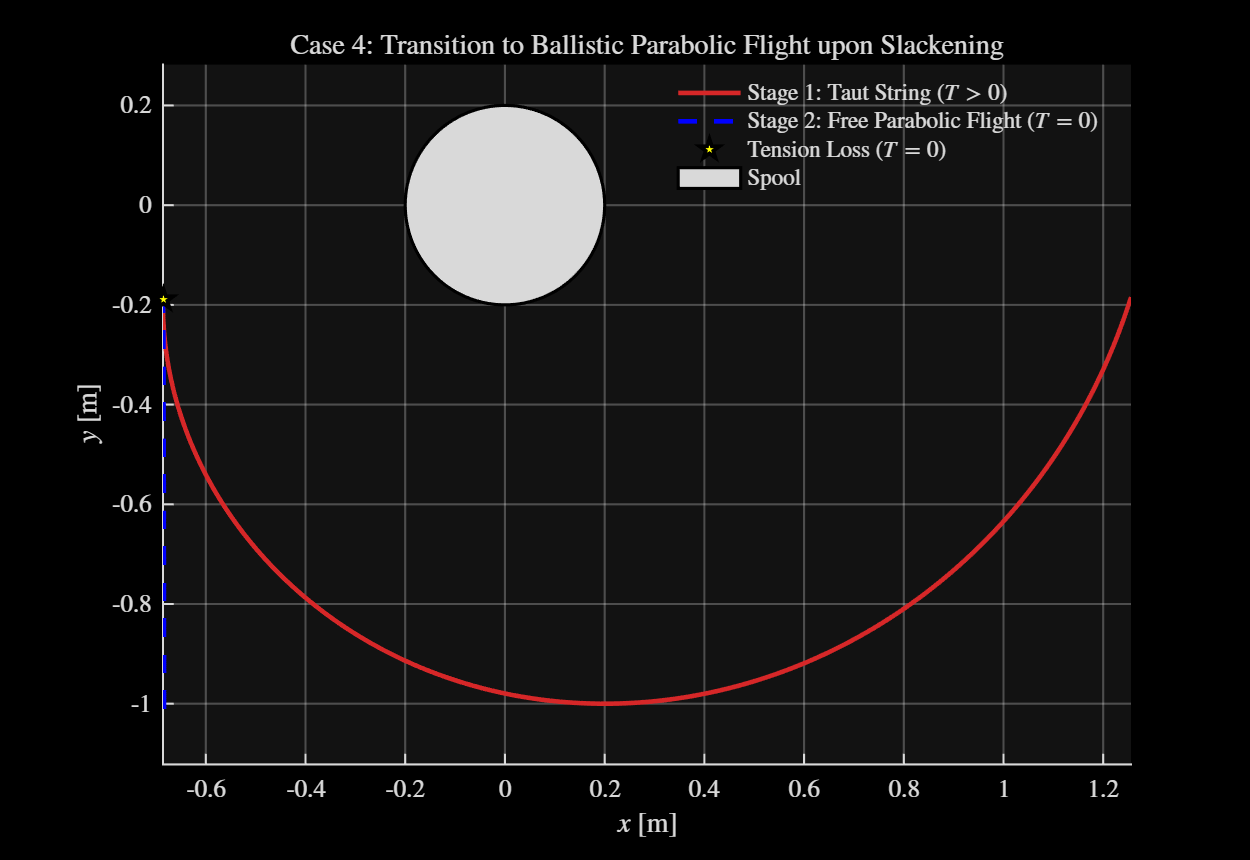
\includegraphics[width=0.68\textwidth]{figs/fig6_case4_ballistic.png}
    \caption{Case 4 trajectory continuation: Stage 1 represents the taut string phase ($T > 0$); Stage 2 demonstrates the ballistic parabolic free fall once tension vanishes at $T = 0$.}
    \label{fig:case4_ball}
\end{figure}

\noindent\textbf{Question 11 Discussion (Post-Slackening Model):} Once $T = 0$, the string can no longer exert constraint forces; the single degree of freedom model becomes physically invalid. To integrate the trajectory beyond $t = 1.6935\text{ s}$:
\begin{enumerate}
    \item Halt the ODE solver at $t_{\text{slack}}$ using \texttt{stopfun}.
    \item Extract the detachment coordinates $\mathbf{r}_P(t_{\text{slack}}) = [-0.680, -0.198]^T\text{ m}$ and velocities $\mathbf{v}_P(t_{\text{slack}}) = [0.012, -0.466]^T\text{ m/s}$.
    \item Switch the governing equations to unconstrained 2D ballistic free fall:
    \begin{equation}
        \ddot{x} = 0, \qquad \ddot{y} = -g.
    \end{equation}
    \item Terminate ballistic flight when the distance from particle $P$ to the tangency point again equals the slack string length, resulting in a sudden inelastic jerk that re-tauts the string.
\end{enumerate}

\subsubsection{Case 5: Multi-Cycle Rheonomic Winding ($\omega = 0.1\text{ rad/s}, \dot{x}_P(0) = +1.0\text{ m/s}$)}
Case 5 combines active spool rotation with an initial swing. Over 35 seconds, the particle executes multiple back-and-forth oscillations. However, because $\omega > 0$, string is continuously wound around the spool on average. The natural frequency $\omega_n \approx \sqrt{g/\xi}$ steadily increases as the pendulum length shortens. Eventually, at $t = 35.5094\text{ s}$, the straight segment is fully wound ($\xi \to 0$), and the particle strikes the spool at $\phi = -1.444\text{ rad}$. The stop condition is **Event 1 (hitting the spool)**.

---

\section{Conclusions}
\label{sec:conclusions}

This study has investigated the dynamics of a particle tethered to a rotating spool through rigorous analytical formulation and numerical simulations in MATLAB. The principal scientific conclusions are:
\begin{enumerate}
    \item \textbf{Decoupled Formulation:} Projecting Newton's Second Law onto the moving normal direction $\mathbf{n}$ successfully decouples the angular acceleration $\ddot{\phi}$ from the unknown string tension $T$, producing a second-order nonlinear ODE that describes the system's single configuration degree of freedom.
    \item \textbf{Energy Theorem Verification:} Numerical simulations confirmed the fundamental theorem of constraints: for scleronomic spools ($\omega = 0$), the tension force performs zero work and mechanical energy is strictly conserved. For rotating spools ($\omega \neq 0$), the rheonomic constraint performs non-conservative work at rate $P = a\omega T(t)$, causing monotonic energy growth.
    \item \textbf{Singularity Dynamics (Case 3):} When $\xi \to 0$, the collapse of the local moment of inertia $m\xi^2$ forces the angular velocity to diverge asymptotically ($|\dot{\phi}| \to \infty$). Setting a physical contact threshold $\epsilon_{\text{contact}}$ within \texttt{stopfun} is essential to avoid numerical solver breakdown.
    \item \textbf{Discontinuous Transitions (Case 4):} When gravity overcomes centripetal acceleration, tension vanishes ($T \to 0$). Simulating the subsequent motion requires a multi-stage solver architecture transitioning from a 1-DOF polar ODE to a 2-DOF Cartesian ballistic flight model.
\end{enumerate}

---

\bibliographystyle{IEEEtran}
\bibliography{references}

\end{document}
